\chapter{The oghma file format}

\section{the .oghma simulation file format}
\label{sec:fileformat}
In OghamNano simulations are saved in a directory containing a sim.oghma file. All the parameters specifying the device and simulations are stored in the sim.oghma file. If you rename the file so to be called sim.zip you will be able to open it in windows explorer or your favourite zip viewer.  Inside the .oghma file you will find another file called sim.json. You can view this file in any text editor but the file is quite long so I recommend you use firefox as it has a very nice built in json viewer.  Json is a simple way of storing text and configuration information first developed for Java. Json is a standard way to store and transmit data much like XML. You can see examples here: \url{https://json.org/example.html} or below in code listing \ref{json-example}.
\linebreak
\linebreak
\vspace{0pt}
\begin{minipage}[]{0.5\textwidth}
You can see the json file is structured using a series of brackets, double quotes and commas. If you make a copy of sim.json outside the .oghma archive, then rename the sim.zip back to sim.oghma, OghmaNano will ignore the sim.json file within the sim.oghma archive and revert to the plain text file stored in the simulation directory.  This feature can be useful for automation of simulations as you can simply edit the sim.json file using your favourite programming language without having to learn about reading and writing zip files. If you open the sim.json file in firefox it will look like \ref{fig:jsonfirefox}.  Also have a look at the file in notepad to get a sense of what is in it.
\end{minipage}% Don't leave empty lines and empty chars between minipages
\begin{minipage}[]{0.5\linewidth}
\begin{minted}[frame=single,
               framesep=3mm,
               linenos=true,
               xleftmargin=21pt,
               tabsize=4]{js}
{
  "color_of_dog": "brown",
  "dog_age": 5,
  "dogs_toys": {
				"rabbit": "True",
				"stick": "False"
				}

}
\end{minted}
\captionof{figure}{A simple JSON example} 
\label{json-example}
\end{minipage}

You can see that the json file has various headings, key headings are listed below in table \ref{fig:jsontab}. If you wish to programmatically drive OghmaNano you can simply use one of the many available json editors most languages have them freely available.

\begin{figure}
\centering
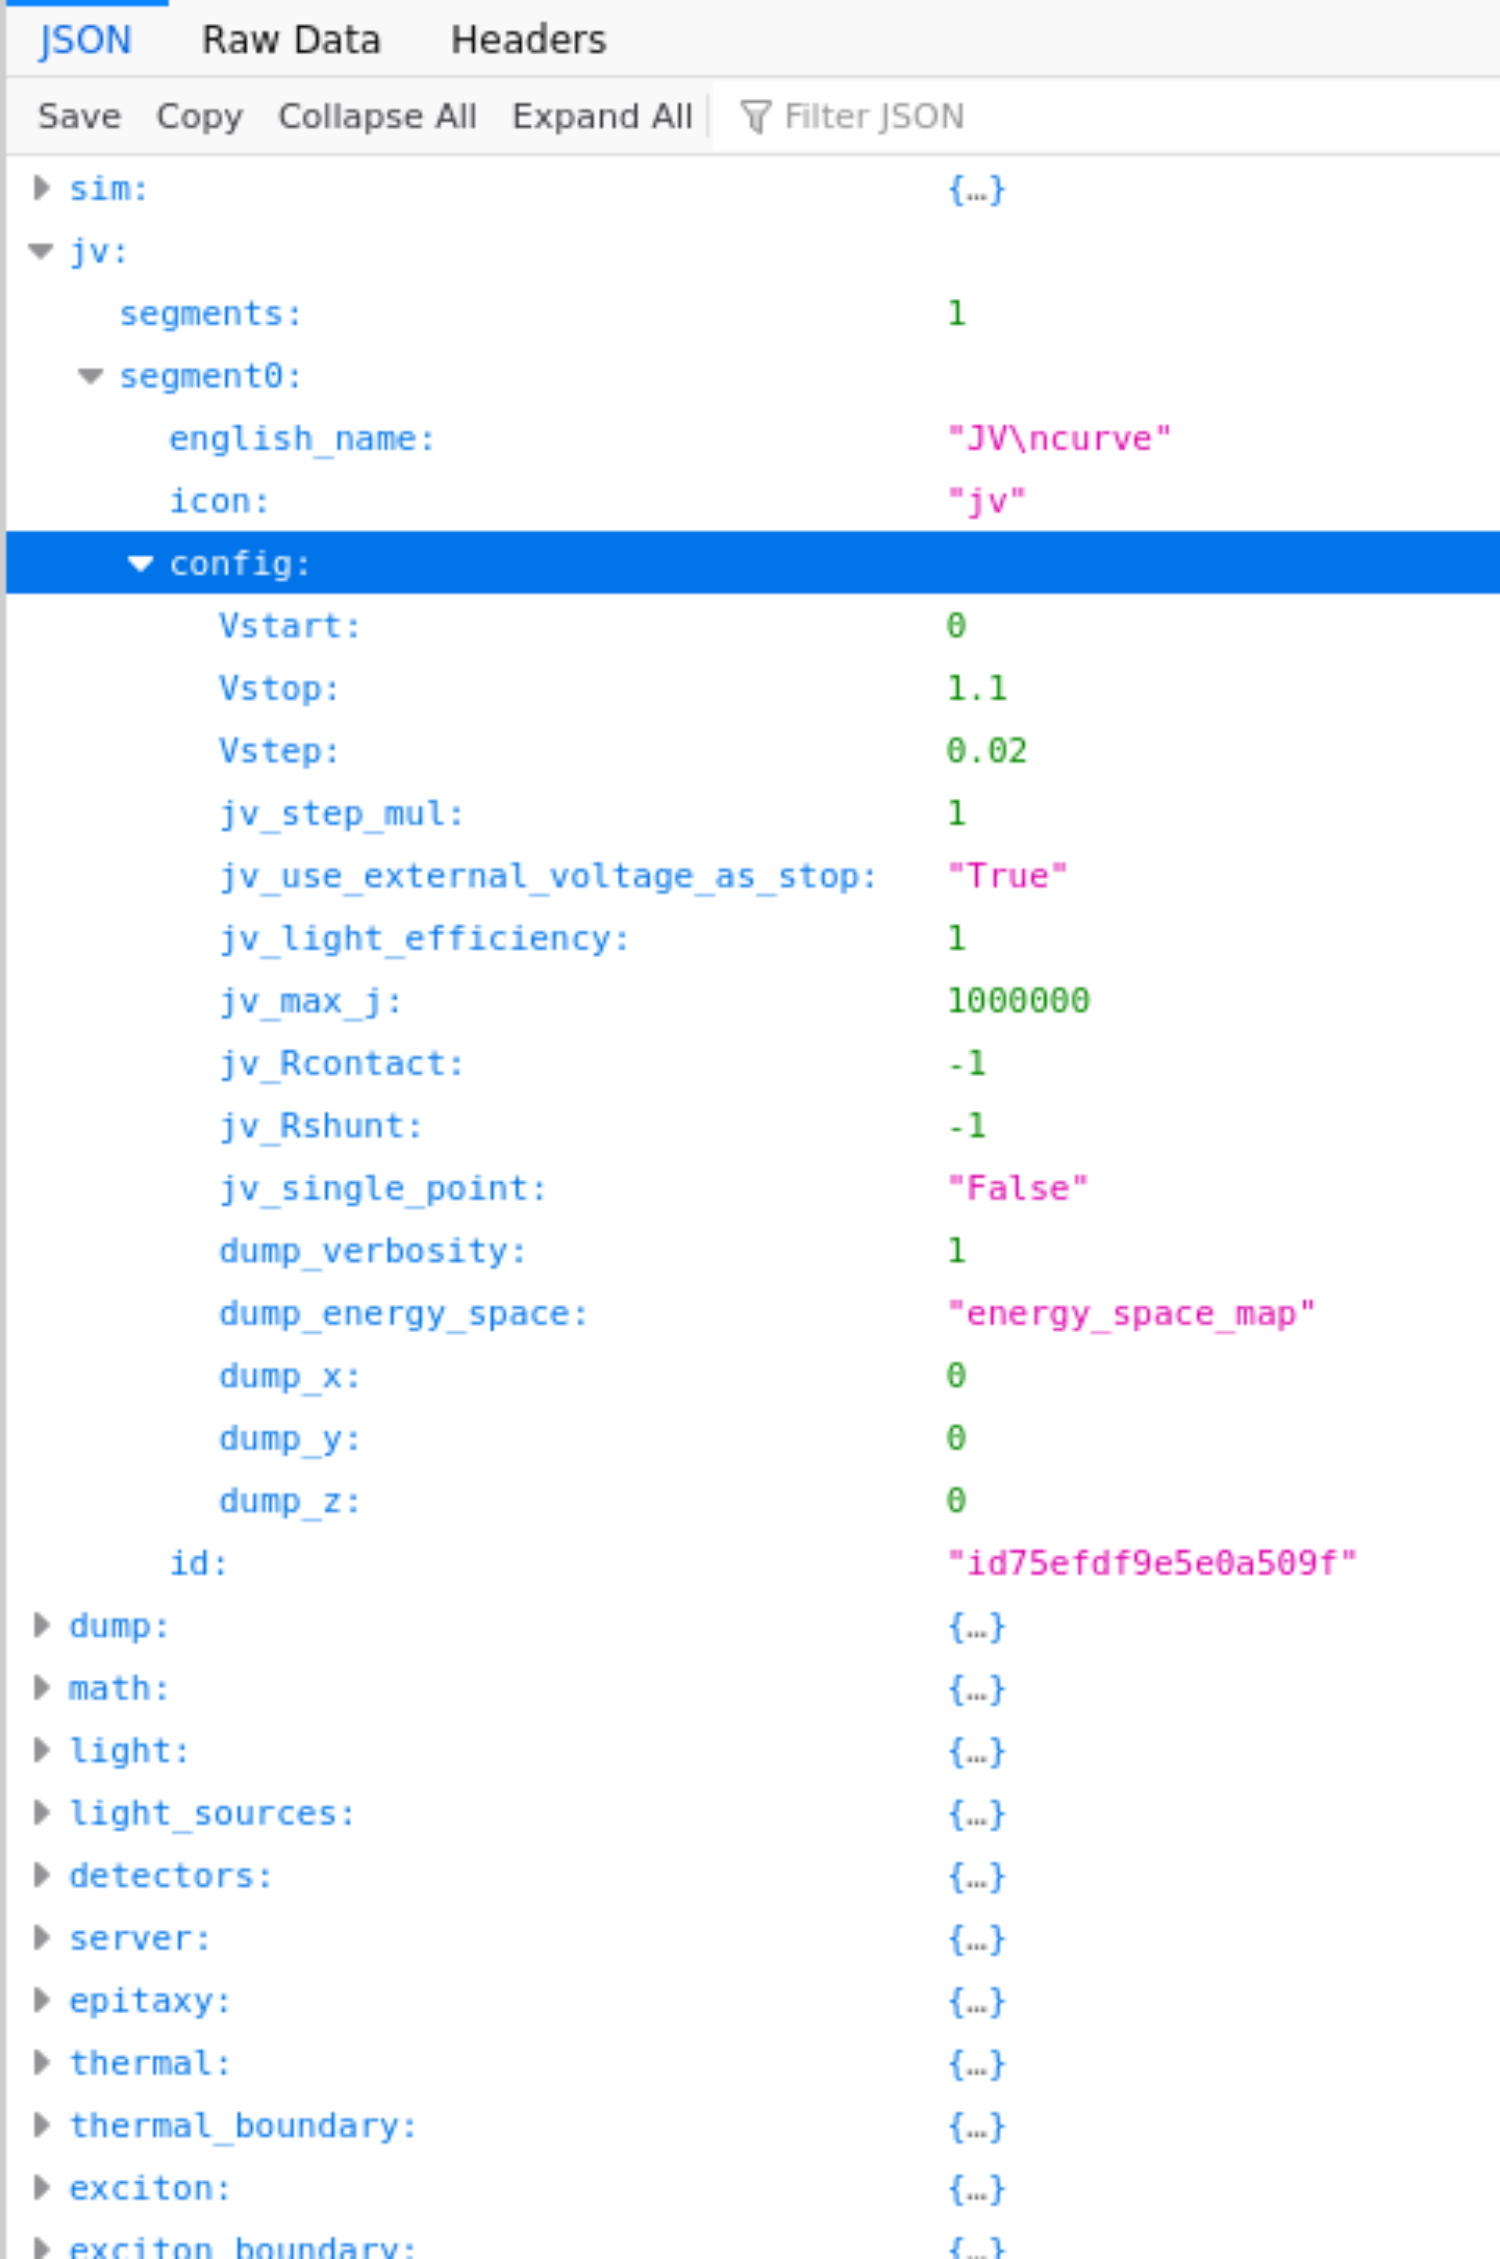
\includegraphics[width=0.55\textwidth]{./images/json_firefox.png}
\caption{An example sim.json file opened in Firefox.}
\label{fig:jsonfirefox}
\end{figure}

\begin{table}
\begin{center}
\begin{tabular}{ |c|c| } 
 \hline
	Heading 			& 	Description  \\ 
 \hline
	sim					&	General simulation information \\
	jv					&	JV curve configuration \\
	dump				&	Defines how much information is written to disk \\
	math				&	Math configuration for the solver \\
	light				&	Optical transfer matrix configuration \\
	light\_sources		&	Configuration of light sources\\
	epitaxy				&	Defines the structure of the device\\
	thermal				&	Thermal configuration\\
	thermal\_boundary	&	Thermal boundary config.\\
	exciton				&	Exciton config\\
	exciton\_boundary	&	Exciton boundary config. \\
	ray					&	Ray tracing config.\\
	suns\_voc			&	Suns-Voc\\
	suns\_jsc			&	Suns-Jsc\\
	ce					&	Charge Extraction config.\\
	transfer\_matrix	&	Light transfer matrix config\\
	pl\_ss				&	PL in steady state\\
	eqe					&	EQE config.\\
	fdtd				&	FDTD config.\\
	fits				&	Fitting config.\\
	mesh				&	Electrical mesh config.\\
	time\_domain		&	Time domain config.\\
	fx\_domain			&	FX-domain config\\
	cv					&	CV config.\\
	parasitic			&	Parasitic components\\
	spm					&	Scanning Probe Microscopy config.\\
	hard\_limit			&	Setting hard limits for sim params.\\
	perovskite			&	Perovskite solver config.\\
	electrical\_solver	&	Electrical solver config.\\
	spctral2			&	SPCTRAL2\\
	lasers				&	fs Lasers \\
	circuit				&	Circuit solver config.\\
	gl					&	OpenGL config\\
	world				&	Defines the world box\\
 \hline
\end{tabular}
\caption{Key headings/sections in the sim.json file.}
\label{fig:jsontab}
\end{center}
\end{table}


\section{Qwerks of the OghmaNano json format}
\begin{itemize}
  \item The OghmaNano json file does not support standard json lists e.g. ["Red", "Green", "Blue"].  If there is a list of items, it is defined by firstly declaring the variable segments, with the number of items in the list so for example "segments",0 . Each item in the list is then stored under, "segment0", "segment1" etc... This format enables OghmaNano to allocate the memory for reading in the structures before doing the reading.  This can be seen in figure \ref{fig:jsonfirefox} where there is a list with 1 segment.
  \item Many items in the json file will be given an ID number which is a 16 digit hex code, this can be used to uniquely reference the item.  An ID number can also be seen in figure \ref{fig:jsonfirefox}.  These ID numbers are generated at random but every ID number must be unique. ID numbers enable objects for example epitaxy layers to be identified uniquely even if they have the same name.
\end{itemize}

\section{Encoding}
The .json files read/written by OghamNano are always stored in \href{https://en.wikipedia.org/wiki/UTF-8}{UTF-8} format. OghmaNano can not handle UTF-16 or any other text encoding standards. Nowadays windows notepad and most other apps default to UTF-8, so if you don't know what these text storage formats are it probably does not matter. This will only rear it's head if you start programmatically generating .oghma files in a language such as C++ and are using a language such as Chinese or Russian with non Latin characters in it's alphabet.

\section{Forwards/backwards compatability of the file format}
Significant effort is made to make sure new versions of OghmaNano can read files generated in older versions. However, older versions of OghmaNano may not be able to read files generated on newer versions. Every time the user opens a sim.oghma file using the GUI the file format is checked and if it differs to that being used in the current version the file is updated and written back to disk. If you are using OghmaNano in a headless configuration by calling $oghma\_core.exe$ directly, then when sim.oghma files from old versions of the model, before running $oghma\_core.exe$, make sure you have opened it in the GUI first to make sure the file is in the correct format.








